\documentclass[a4paper,12pt,fleqn]{article}
\setlength{\mathindent}{0pt}% Remove indentation
\usepackage{amsmath}
\usepackage{listings}
\usepackage{xcolor}
\usepackage{hyperref}
\usepackage{graphicx}
\usepackage{subcaption}


\begin{figure}[h]
    \centering
    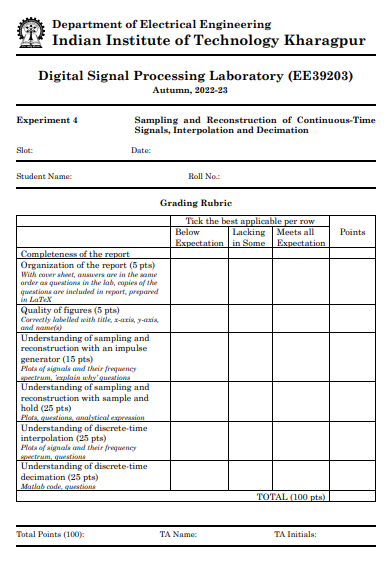
\includegraphics[width=1\linewidth]{firstpg.png}
    \label{fig:enter-label}
\end{figure}

\title{Digital Signal Processing Laboratory (EE39203)\\ Experiment 1: Discrete and Continuous-Time Signals}
\author{Name: Sujay Vivek \\
Roll Number: 22EE30029}
\date{August 7th 2024}

\lstset{
    language=Matlab,           % Choose the language of the code
    basicstyle=\ttfamily,      % The font style to use for the code
    keywordstyle=\color{violet}, % Color of keywords
    commentstyle=\color{green},% Color of comments
    stringstyle=\color{blue},   % Color of strings
    numbers=left,              % Where to put line numbers
    numberstyle=\tiny\color{black}, % Style for line numbers
    stepnumber=1,              % Step between two line numbers
    numbersep=10pt,            % Distance between line numbers and code
    backgroundcolor=\color{white}, % Background color of the code block
    showspaces=false,          % Show spaces as dots
    showstringspaces=false,    % Do not show spaces in strings
    frame=single,              % Add a frame around the code
    breaklines=true,           % Allow line breaking
    breakatwhitespace=true,    % Break lines at whitespace
    tabsize=4,                 % Set the size of tabs
    captionpos=b               % Set caption position to bottom
}


\begin{document}
\newpage
\maketitle  % Place the title here to ensure it appears before the figure



% Add more content here if needed
\section*{1. Learning Objective}
This lab aims to demonstrate the characteristics of continuous and discrete-time signals using digital computers and the MATLAB software environment. A 
continuous-time signal takes on a value at every point in time, whereas a discrete-time signal is only defined at integer values of the “time” variable. However, while discrete-time signals can be easily stored and processed on a computer, storing the values of a continuous-time signal for all points along a segment of the real line is impossible. In this experiment, we will illustrate that continuous-time signals can be processed by first approximating them as discrete-time signals through sampling.


\section*{3. Continuous-Time Vs. Discrete-Time}

\subsection*{3.1 Displaying Continuous-Time Vs. Discrete-Time}
To plot discrete-time signals as dots in a Cartesian coordinate system, the MATLAB \texttt{stem} command is used. Multiple plots on a single figure can be managed using the \texttt{subplot} command. Continuous-time signals can be approximated by computing their values at closely spaced points in time and plotting these with connecting lines using the \texttt{plot} function in MATLAB.

\newpage
\subsection*{\underline{MATLAB Code}}
\begin{lstlisting}
% Defining the function

f = @(t) sin(t).*sin(t);

% Creating Sampling Frequencies
Fs1 = 5;
Fs2 = 10;
Fs3 = 20;

% Creating Discrete Time values
t_continuous = linspace(0,10,1000); 

t_discrete1 = 0:1/Fs1:10;   % Sampling Freq = 5
t_discrete2 = 0:1/Fs2:10;   % Sampling Freq = 10
t_discrete3 = 0:1/Fs3:10;   % Sampling Freq = 20

% Calculating the function values
y_cont = f(t_continuous);
y_disc1 = f(t_discrete1);
y_disc2 = f(t_discrete2);
y_disc3 = f(t_discrete3);

% Create the subplot for the continuous plot
subplot(4, 1, 1);
plot(t_continuous, y_cont);
title('Continuous Plot of f(t) = sin(t) * sin(t)');
xlabel('Time (t)');
ylabel('f(t)');
grid on;

% Create the subplot for the discrete plot with Fs1
subplot(4, 1, 2); 
stem(t_discrete1, y_disc1);
title('Discrete Plot of f(t) with Sampling Freq = 5');
xlabel('Time (t)');
ylabel('f(t)');
grid on;

% Create the subplot for the discrete plot with Fs2
subplot(4, 1, 3);
stem(t_discrete2, y_disc2);
title('Discrete Plot of f(t) with Sampling Freq = 10');
xlabel('Time (t)');
ylabel('f(t)');
grid on;

% Create the subplot for the discrete plot with Fs3
subplot(4, 1, 4);
stem(t_discrete3, y_disc3);
title('Discrete Plot of f(t) with Sampling Freq = 20');
xlabel('Time (t)');
ylabel('f(t)');
grid on;

sgtitle('Sujay Vivek - 22EE30029');

\end{lstlisting}

\FloatBarrier  % Ensures that the new subsection starts on a new page
\newpage

\subsection*{\underline{Plots}}
Plotting with the help of MATLAB:
\begin{figure}[h]
    \centering
    % First plot
    \begin{subfigure}{1.15\textwidth} % 115% of the text width
        \centering
        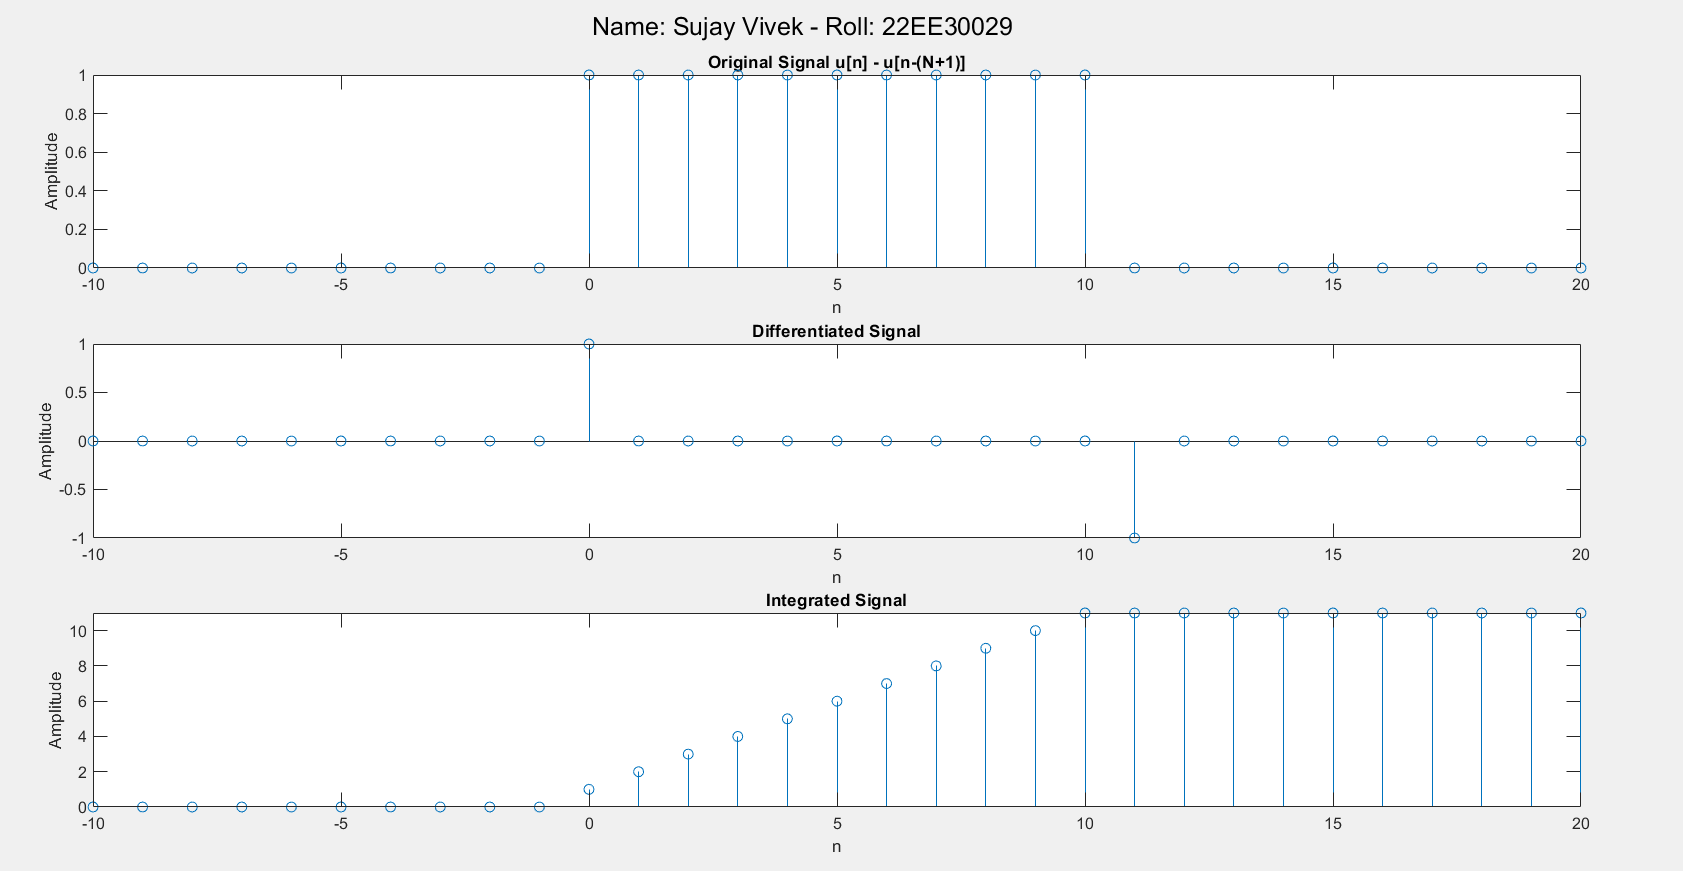
\includegraphics[width=\linewidth]{1.png}
        \caption{Continous and Discrete Plots of f(t) using different Sampling Frequencies}
        % \label{fig:sineplot}
    \end{subfigure}
    \hfill % Horizontal space between the figures
   
\end{figure}

\subsection*{\underline{Observation:}}
Looking at the above generated waveforms of different sampling frequencies, we can easily comment that the Continuous Time Plot is accurate as we have computed large number of values at closely spaced points in time. 

The Discrete time waveform however has less number of computed values and hence there is less accurate compared to the continuous time plot. One can observe that as the Sampling Frequency reduces, the number of computed points on the waveform also reduces.

\FloatBarrier  % Ensures that the new subsection starts on a new page
\newpage  % Start a new page

\subsection*{3.2 Vector Index vs. Time}
In MATLAB, vector indices start from 1 and cannot be negative or zero. When sampling a continuous-time signal like \( x(t) \), it's common to store these samples in a vector, often using the same variable name (e.g., \( x[n] \)). However, it's important to differentiate between the vector index \textbf{ x[n]} and the function \textbf{x(t)}, as they are distinct concepts despite potentially sharing the same name.

\subsection*{\underline{MATLAB Code}}
\begin{lstlisting}

% Creating a function to make things easier
function a = create_disc(gap)
    a = 0:gap:10;
end

% Define the new function to be plotted
f = @(t) cos(t).*cos(t);

% Generate discrete time points with different sampling intervals
t_disc1 = create_disc(0.1);
t_disc2 = create_disc(0.5);
t_disc3 = create_disc(0.9);

% Calculate the function values at the discrete time points
y_disc1 = f(t_disc1);
y_disc2 = f(t_disc2);
y_disc3 = f(t_disc3);

% Create the first subplot with sampling interval 0.1
subplot(3, 1, 1); 
stem(t_disc1, y_disc1);
title('Discrete Plot of f(t) = cos(t) * cos(t) with Sampling Interval = 0.1');
xlabel('Time (t)');
ylabel('f(t)');
grid on;

% Create the second subplot with sampling interval 0.5
subplot(3, 1, 2); 
stem(t_disc2, y_disc2);
title('Discrete Plot of f(t) = cos(t) * cos(t) with Sampling Interval = 0.5');
xlabel('Time (t)');
ylabel('f(t)');
grid on;

% Create the third subplot with sampling interval 0.9
subplot(3, 1, 3); 
stem(t_disc3, y_disc3);
title('Discrete Plot of f(t) = cos(t) * cos(t) with Sampling Interval = 0.9');
xlabel('Time (t)');
ylabel('f(t)');
grid on;

% Add a supertitle for the figure
sgtitle('Sujay Vivek - 22EE30029');


\end{lstlisting}
\FloatBarrier
\newpage
\subsection*{\underline{Plots}}
\begin{figure}[h]
        \centering
        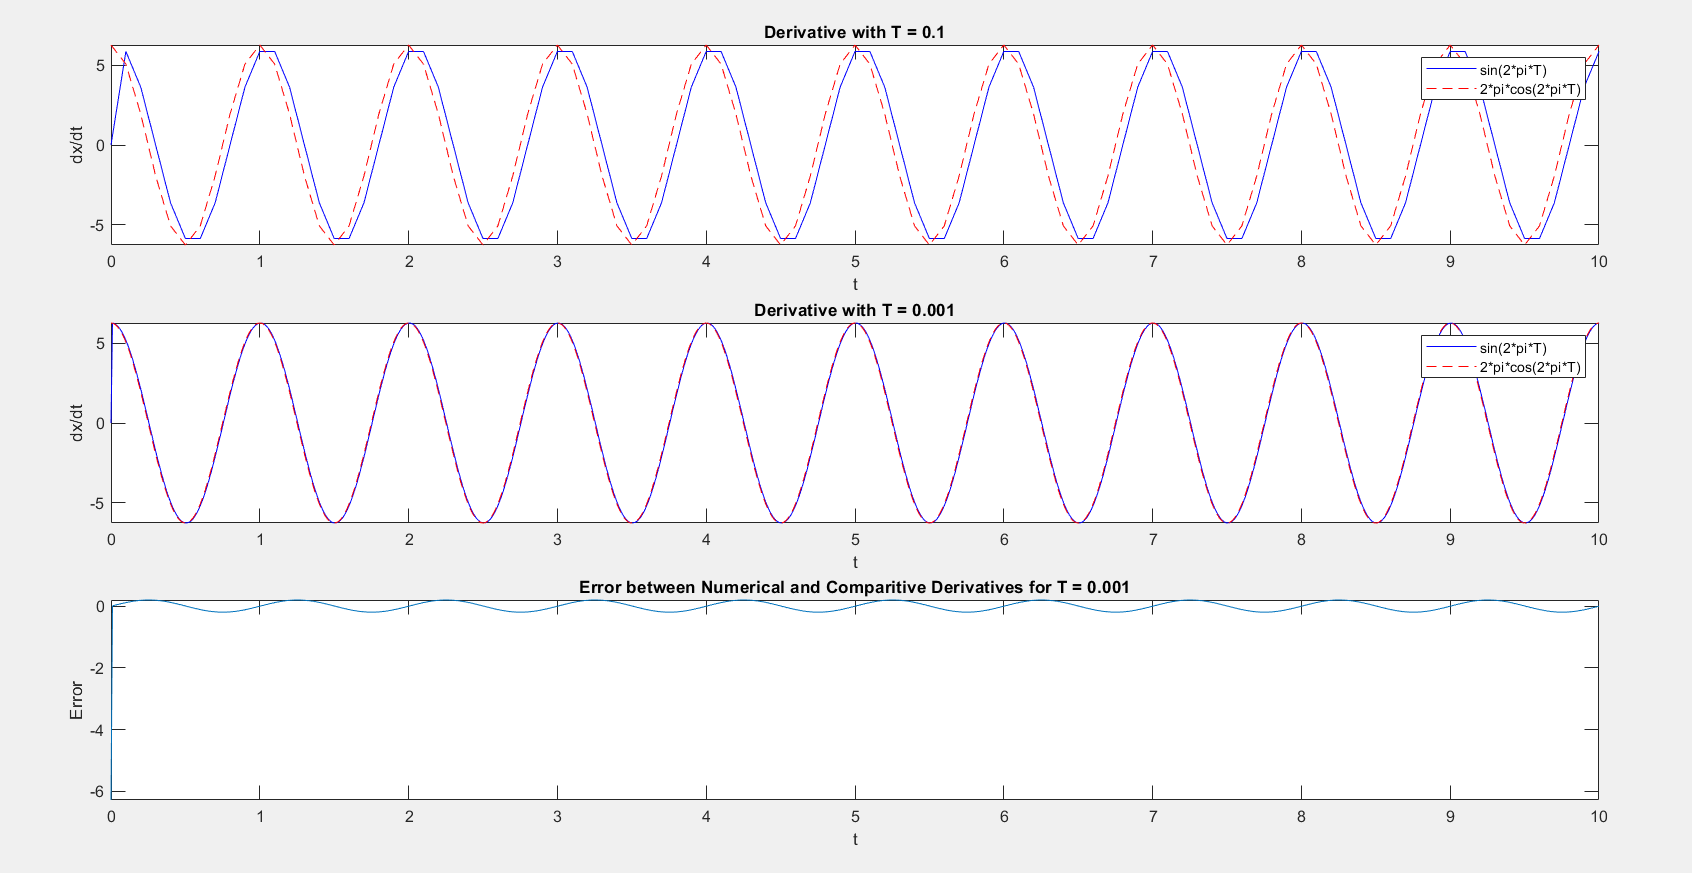
\includegraphics[width=1\linewidth]{2.png}
        \caption{Plotting f(t) at different Sampling Intervals}
        \label{fig:enter-label}
\end{figure}

\subsection*{\underline{Observation:}}
Observing each of the 3 graphs above, we can notice how Sampling Frequency affects the Generated Waveform of the function f(t). 
The Waveforms depict the use of Sampling Time Intervals 0.1, 0.5 and 0.9 top to bottom. And we observe that as the Sampling Time Intervals increase, the number of discrete points computed and displayed on the Waveform decreases, and hence the accuracy also decreases.


\newpage
\subsection*{3.2 Graphing a Sine Wave for a particular Range}
Writing Matlab command(s) that would print the graph of sin(t) for the values of t on the interval [3.5, 4.5] for an appropriate increment of t.



\subsection*{\underline{MATLAB Code}}
\begin{lstlisting}
%Now trying to print the sin curve within a given interval
 f = @(t) sin(t);
   a = 3.5;
   b = 4.5;

%Creating the time values
t_c = linspace(a,b,1000);

y3 = f(t_c); 
%Getting the output in y3 for each of the time values
plot(t_c, y3);

title(["Continous plot of sin(t) in the interval 3.5 to 4.5","Name: Sujay Vivek, Roll No: 22EE30029"]);

xlabel('Time (t)');
ylabel('f(t) = sin(t)');
grid on;

\end{lstlisting}
\subsection*{\underline{Plots}}
Plots generated by MATLAB:
\newline


    \begin{subfigure}{1.15\textwidth} % 115% of the text width
        \centering
        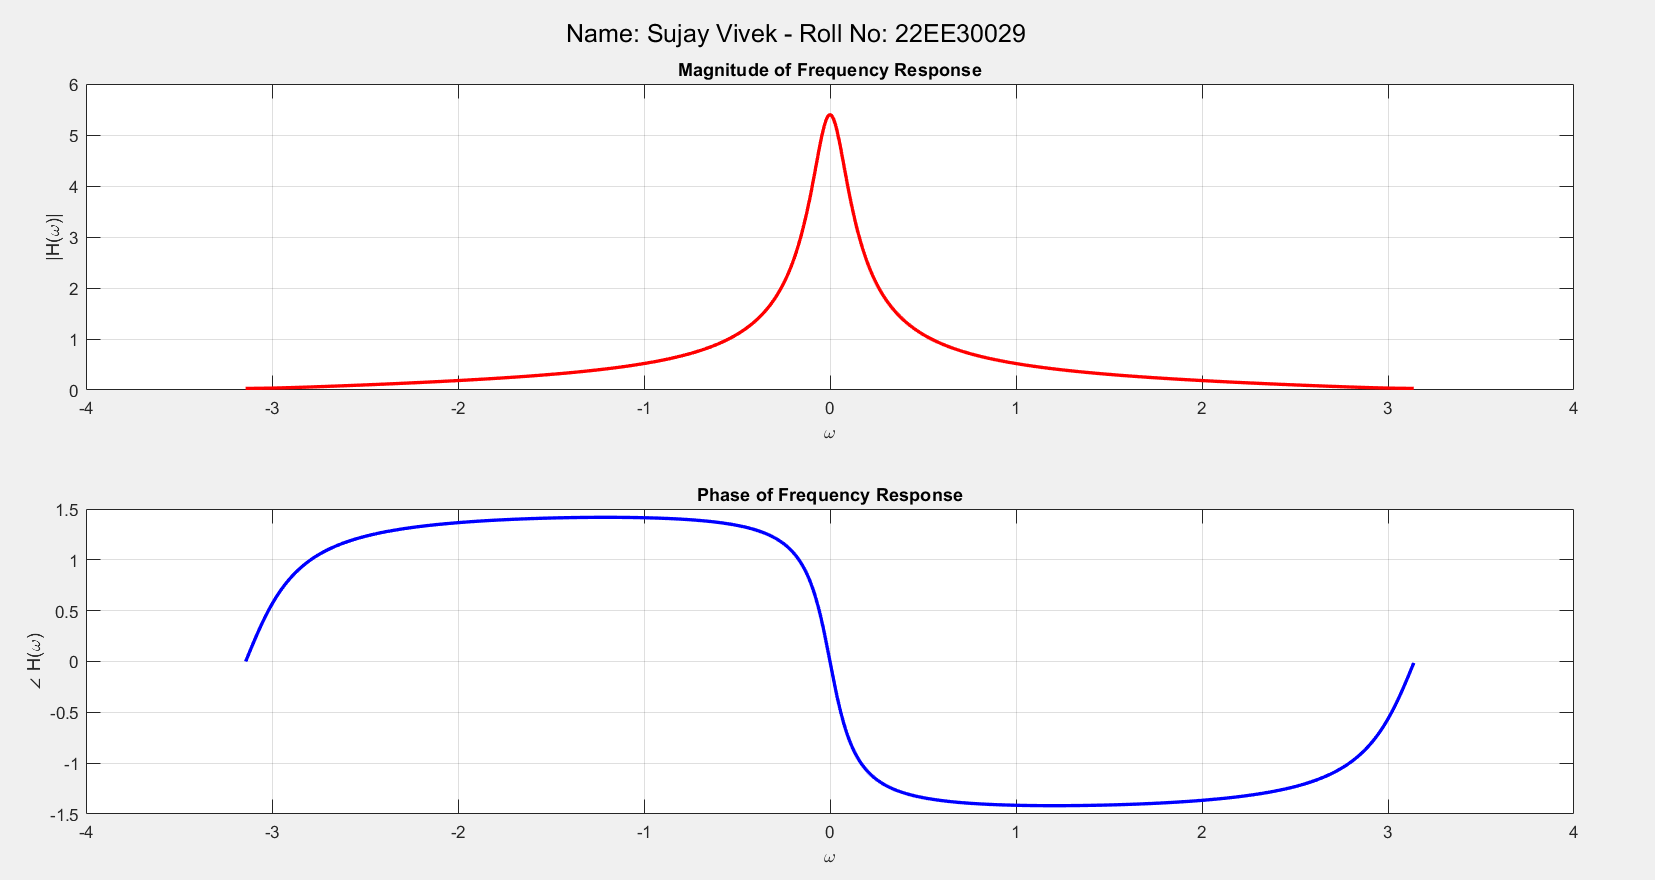
\includegraphics[width=\linewidth]{3.png}
        \caption{Graph of Sine Wave in [3.5,4.5]}
    \end{subfigure}

% \subsection*{\underline{Plots}}
% \begin{figure}[h]
%         \centering
%         \includegraphics[width=1\linewidth]{plot_vector.png}
%         \label{fig:enter-label}
% \end{figure}


\subsection*{2.3 Analytical Calculation}
Computing the following integrals manually:
\begin{equation*}
x_1(t) = \int_0^{2\pi} \sin^2(7t) \, dt
\end{equation*}
\begin{equation*}
x_2(t) = \int_0^1 e^t \, dt
\end{equation*}
\\ \\
Answer:
\newline
\begin{equation}
\begin{split}
x_1(t) & = \int_{0}^{2\pi} \sin^2(7t) \, dt \\
& = \int_{0}^{2\pi} \frac{1 - \cos(14t)}{2} \, dt \\
& = \frac{1}{2} \int_{0}^{2\pi} (1 - \cos(14t)) \, dt \\
& = \frac{1}{2} \left[ \int_{0}^{2\pi} 1 \, dt - \int_{0}^{2\pi} \cos(14t) \, dt \right] \\
& = \frac{1}{2} \left[ t \Big|_{0}^{2\pi} - \frac{\sin(14t)}{14} \Big|_{0}^{2\pi} \right] \\
& = \frac{1}{2} \left[ 2\pi - 0 \right] \\
& = \pi \\
\end{split}
\end{equation}

\begin{equation}
\begin{split}
x_2(t) & = \int_{0}^{1} e^t\,dt\\
  & = \left[ e^t \right]_{0}^{1}\\
  & = e^1 - e^0\\
  & = e - 1\\
\end{split}
\end{equation}
\newpage

\subsection*{3.4  Numerical Computation of Continuous-Time Signals}
In this section, we will numerically compute integrals using the Riemann method. The Riemann integral approximates the area under a curve by breaking the region into many rectangles and summing their areas. Each rectangle is chosen to have the same width Δt, and the height of each rectangle is the value of the function at the start of the rectangle’s interval. We will create MATLAB functions to approximate the integral of \( \mathbf{sin^2(7t)} \) over \([0, 2\pi]\) and \( \mathbf{exp(t)} \) over \([0, 1]\), using varying numbers of rectangles. The function will avoid loops and use the \texttt{sum} command. 

We will also plot how the approximation improves with more rectangles.



\subsection*{\underline{MATLAB Code}}
\begin{lstlisting}
function I = integ1(N)
    t = linspace(0,2*pi,N+1);
    fx = sin(7*t).*sin(7*t);
    t_dif = 2*pi/N;
    I = t_dif*sum(fx(1:end-1));
end

function J = integ2(N)
    t_val = linspace(0,1,N+1);
    fx = exp(t_val);
    t_diff = 1/N;
    J = t_diff*sum(fx(1:end-1));
end

N_vals = 1:100;
I_vals = zeros(size(N_vals));
J_vals = zeros(size(N_vals));

for i=1:length(N_vals)
    I_vals(i) = integ1(i);
    J_vals(i) = integ2(i);
end


% Create the subplot for the continuous plot
subplot(2, 1, 1); % 2 rows, 1 column, 1nd plot in the subplot
plot(I_vals);
title('Integral 1 plotting');
xlabel('N');
ylabel('f(t) = sin(7t)*sin(7t)');
grid on;

% Create the subplot for the continuous plot
subplot(2, 1, 2); % 2 rows, 1 column, 2nd plot in the subplot
plot(J_vals);
title('Integral 2 plotting');
xlabel('N');
ylabel('f(t) = exp(t)');
grid on;

sgtitle('Sujay Vivek - 22EE30029');
\end{lstlisting}

\FloatBarrier  % Ensures that the new subsection starts on a new page
\newpage  % Start a new page

\subsection*{\underline{Plots}}
Include plots of the numerical integration results here.
\begin{figure}[h]
        \centering
        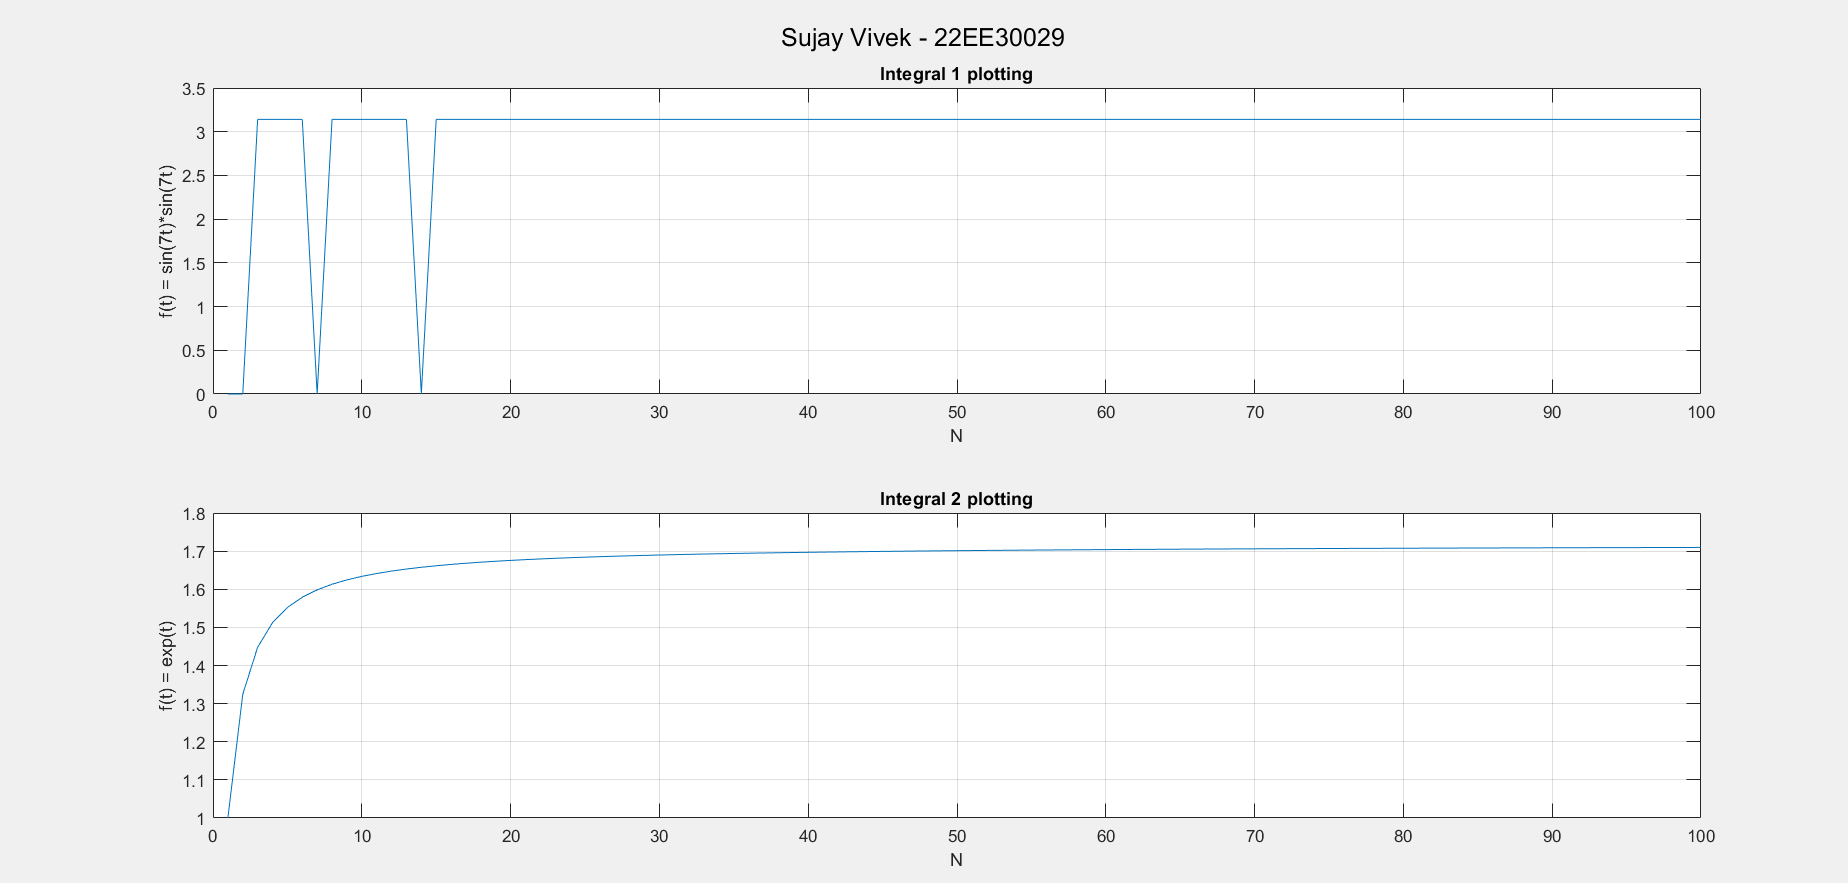
\includegraphics[width=1.1\linewidth]{4.png}
        \caption{Reinmann Integration}
        \label{fig:enter-label}
\end{figure}
\\
Here  I(7) = $4.9 \times 10^{-30}$  and  I(14) = $1.6 \times 10^{-29}$ which is almost = $0$
\\ \\
\textbf{Reason:} When using a method like the rectangular approximation, the interval is divided into N rectangles. I(7) uses 7 rectangles, and I(14) uses 14 rectangles. Obviously, as the number of rectangle increases, we can recreate the function in a much accurate way and hence, we receive more accurate answers as we increase the number of rectangles.

\FloatBarrier
\newpage

\section*{4. Special Functions}
\subsection*{4.1 Plotting Continuous-Time Functions}
Plotting the following continuous-time functions over the given respective intervals.

\begin{equation*}
x_3(t) = \frac{\sin(\pi t)}{\pi t}, \quad t \in [-10, 10]
\end{equation*}
\begin{equation*}
x_4(t) = \text{rect}(t), \quad t \in [-1, 2]
\end{equation*}
 \subsection*{\underline{MATLAB Code}}
 \begin{lstlisting}
g = @(t) sin(pi*t)./(pi*t);  %Function 1

h = @(t) (abs(t)<=0.5);   %Function 2

gx_vals = linspace(-10,10,1000); %creating time intervals
gy_vals = g(gx_vals); %Storing all ouput values in 1 variable

hx_vals = linspace(-1,2,100);
hy_vals = h(hx_vals); %Storing all the points.

% Create the subplot for the continuous plot
subplot(2, 1, 1); % 2 rows, 1 column, 1nd plot in the subplot
plot(gx_vals,gy_vals);
title('function1 plot');
xlabel('time');
ylabel('f(t) = sin(pi*t)/pi*t');
grid on;

% Create the subplot for the continuous plot
subplot(2, 1, 2); % 2 rows, 1 column, 2nd plot in the subplot
plot(hx_vals, hy_vals);
title('function2 plot');
xlabel('time');
ylabel('f(t) = rect(t)');
grid on;

sgtitle('Name: Sujay Vivek, Roll No: 22EE30029');
 \end{lstlisting}
\subsection*{\underline{Plots}}
\begin{figure}[h]
    \centering
    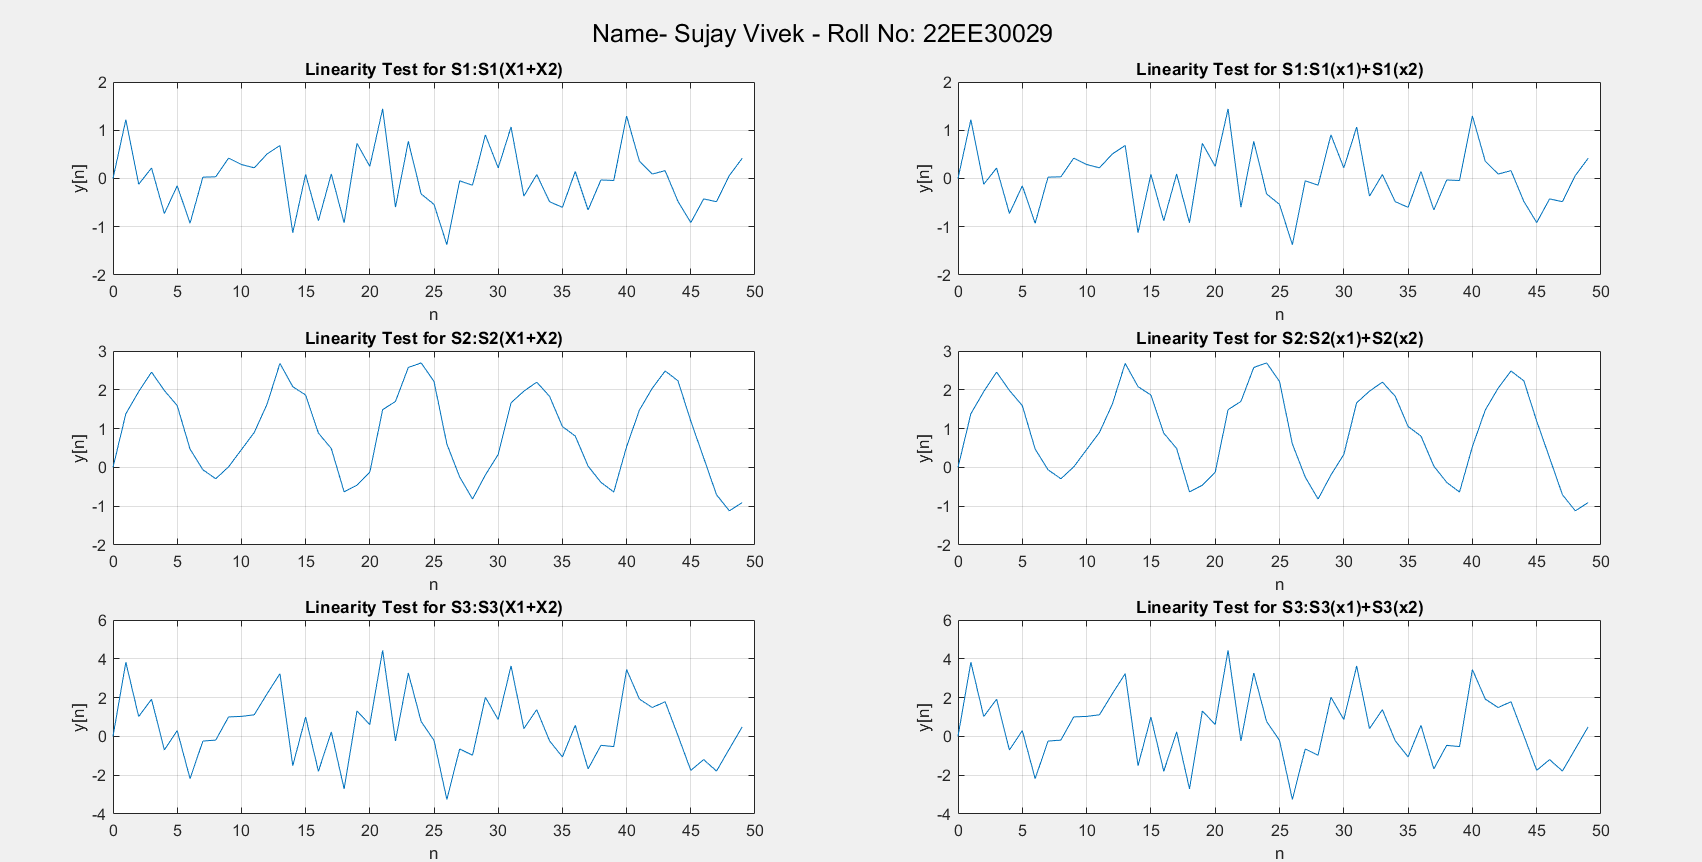
\includegraphics[width=1\linewidth]{5.png}
    \caption{Continuous-time plots of g(t) $ and $ h(t)}
    \label{fig:enter-label}
\end{figure}
\newpage

\subsection*{4.2 Plotting Discrete-Time Functions} 
Plotting the following discrete-time functions over the given respective intervals.
\[
x_1[n] = a^n \left( u[n] - u[n - 10] \right) \quad \text{for } n \in [-20, 20]
\]
\[
x_2[n] = \cos(\omega n) \, a^n u[n] \quad \text{for } \omega = \frac{\pi}{4}, \text{ and } n \in [-1, 10]
\]

\subsection*{\underline{MATLAB Code}}
\begin{lstlisting}
% Discrete-time function x1[n] for different values

% Range of n
n = -20:20; 


u = (n>=0) - (n>=10);

a_values = [0.8, 1.0, 1.5]; %different a values

figure;
orient('tall') %As given the the question for preventing overcrowding of subplots

for i = 1:length(a_values)
    a = a_values(i);
    x1 = a.^n .*u; %Compute x1[n]
    subplot(3,1,i);
    stem(n,x1,'filled');
    title(['Discrete-Time Function x_1[n] for a= ' num2str(a)]);
    grid on;

    sgtitle('Sujay Vivek - 22EE30029');
end


%Discrete-time function x2[n] for omega = pi/4 and different values of a
n2 = -1:10;

u2 = (n2 >= 0);

omega = pi/4;
figure;
orient('tall');

for i = 1:length(a_values)
    a = a_values(i);
    x2 = cos(omega * n2) .* (a .^n2) .*u2;
    subplot(3,1,i);
    stem(n2,x2,'filled');
    xlabel('n');
    ylabel(['x2[n] for a =', num2str(a)]);
    title(['Discrete-Time Function x_2[n] for a =', num2str(a)]);
    grid on;

    sgtitle('Sujay Vivek - 22EE30029');
end

\end{lstlisting}

\subsection*{\underline{Plots}}
\begin{figure}[h]
    \centering
    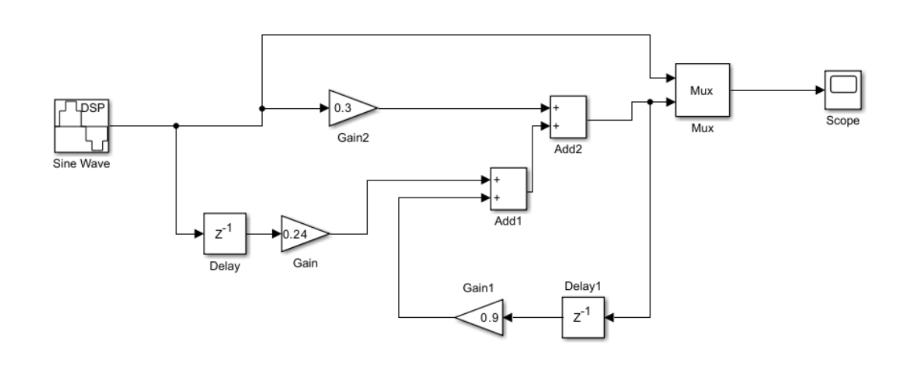
\includegraphics[width=1\linewidth]{6.png}
    \caption{Discrete-time plot of x1[n]}
    \label{fig:enter-label}
\end{figure}

\begin{figure}[h]
    \centering
    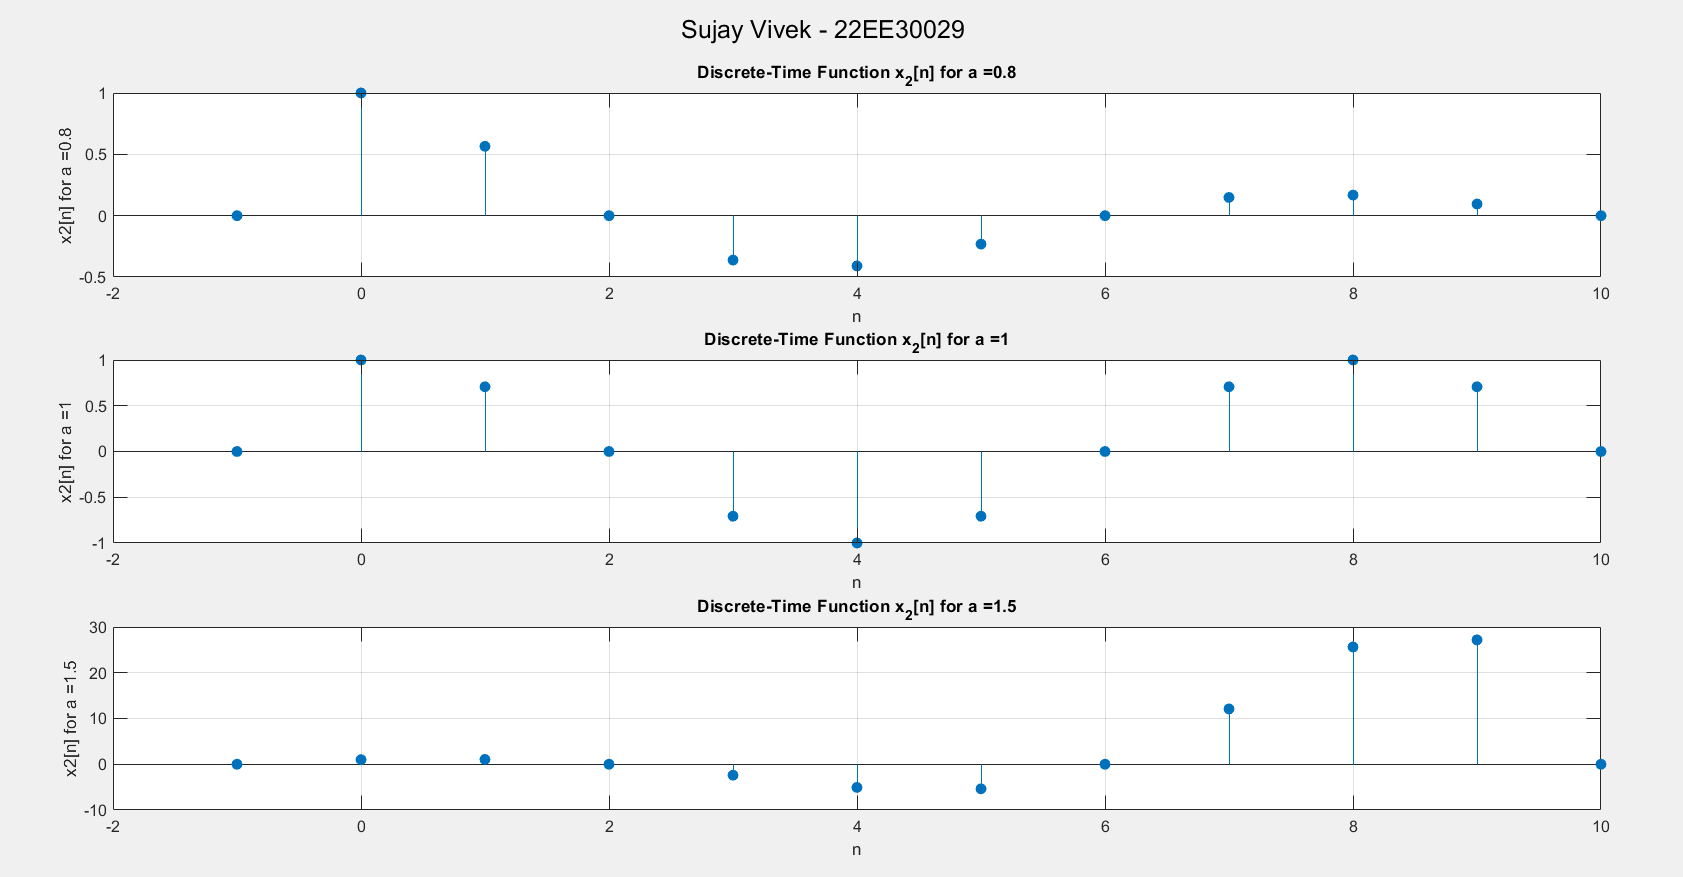
\includegraphics[width=1\linewidth]{7.png}
    \caption{Discrete-time plot of x2[n]}
    \label{fig:enter-label}
\end{figure}
\FloatBarrier
\newpage
\section*{4. Sampling}
In this section, the concept of sampling, which involves converting a continuous-time signal into a discrete-time signal by taking samples at uniformly spaced intervals, is explored. The time between two consecutive samples is called the sampling period. 
For example, a sampling period of 0.1 seconds implies that the value of the signal is stored 
every 0.1 seconds. The signal \( f(t) = \sin(2\pi t) \) is sampled with a period \( T_s \), resulting in a discrete-time signal \( x[n] = \sin(2\pi T_s n) \). The signal is then plotted for various values of \( T_s \) using the \texttt{stem} command, with all plots organized in a single figure via the \texttt{subplot} command.

\subsection*{\underline{MATLAB Code}}
\begin{lstlisting}
% Defining the sampling periods
ts_val = [1/10, 1/3, 1/2, 10/9];

% Define the ranges for n
n_ranges = {0:100, 0:30, 0:20, 0:9};

%Create a new figure
figure;

% Loop through each Ts values
for i = 1:length(ts_val)
    Ts = ts_val(i);
    n = n_ranges{i};

    xn  = sin(2*pi*Ts*n);
    subplot(2,2,i);
    stem(n, xn, 'filled');
    %Labelling the axes and title
    xlabel('n');
    ylabel(['x[n] for T_s =', num2str(Ts)]);
    title(['T_s =', num2str(Ts)]);

    axis([min(n), max(n), -1, 1]);
    grid on;
end

sgtitle('Discrete Time Signal x[n] = sin(2*piT_sn) for Different Sampling Periods');

\end{lstlisting}

\subsection*{Observations:}
\textbf{Ts = 1/10:} The Discrete Time Signal is almost similar to the Continuous Time Signal since the Sample Interval is very small. The generated waveform is quite dense
\\ \\
\textbf{Ts = 1/3:} Larger Sampling period in the case of Ts = 1/3. Hence the waveform generated is a little less denser, though we can make out it is similar to the original continuous waveform.
\\ \\
\textbf{Ts = 1/2:} As the sampling period increases, the number of computed values decreases. The signal is more sparser and less dense.
\\ \\
\textbf{Ts = 10/9:} Here the Ts = 10/9, which is slightly a little more than 1. Hence the number of computed values is very less due to a large Time Interval that is being used for Sampling. Hence the waveform is less dense and very sparse.
\\

\newpage
\subsection*{\underline{Plots}}

\begin{figure}[h]
    \centering
    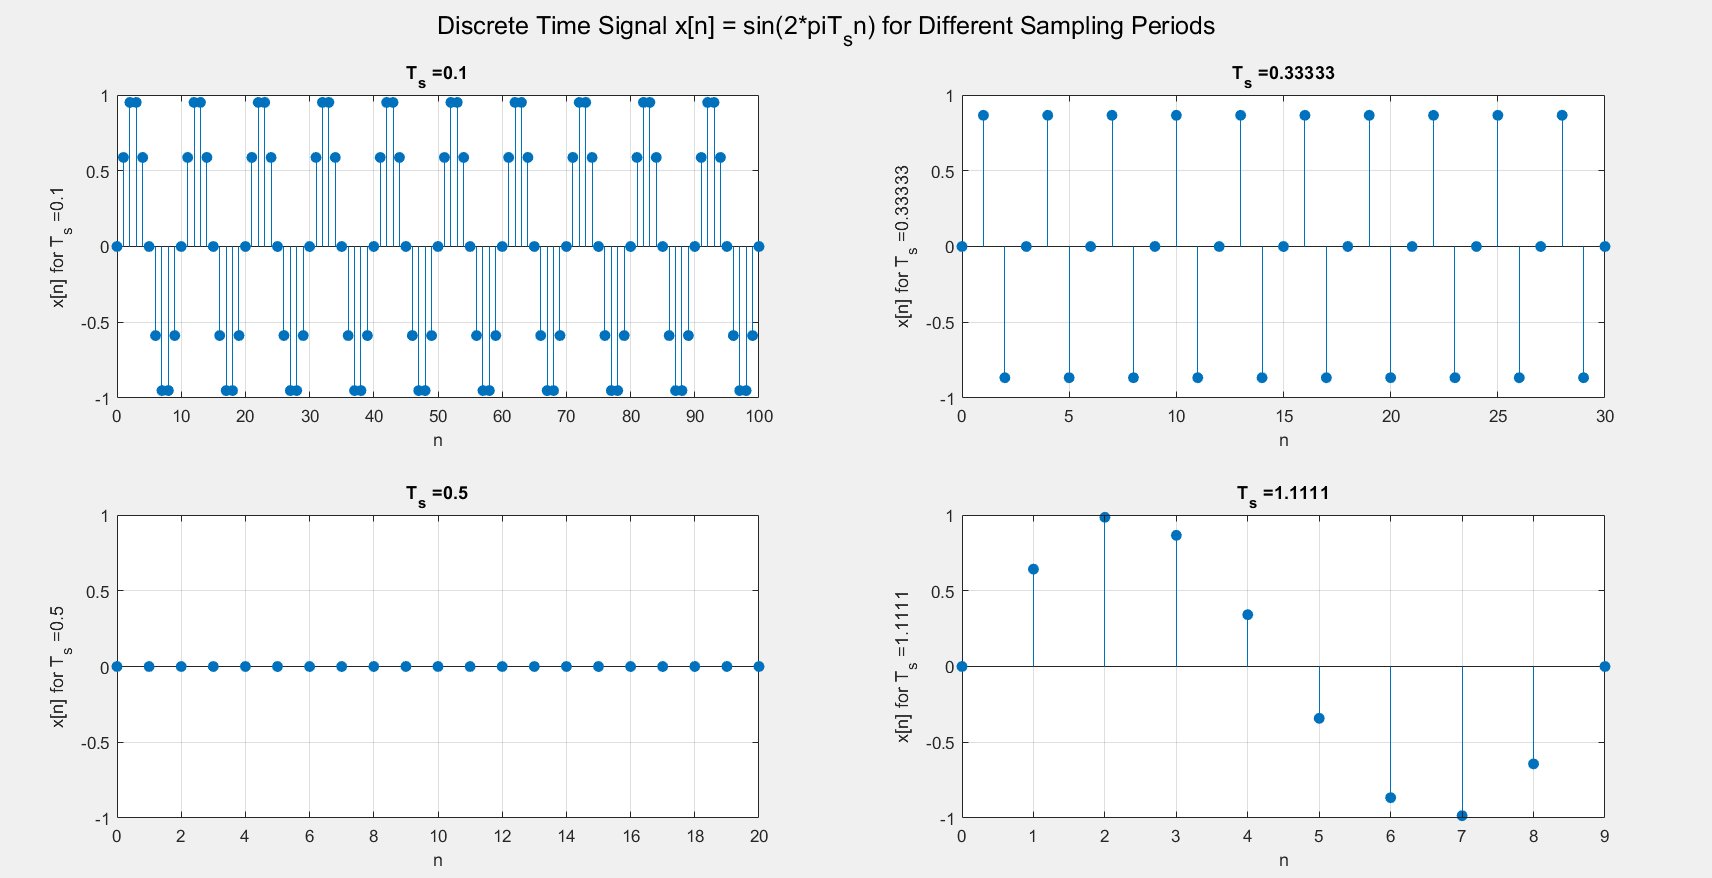
\includegraphics[width=1\linewidth]{8.png}
    \label{fig:enter-label}
\end{figure}

\section*{Understanding}
Sampling in digital communication is converting a continuous-time signal into a discrete-time signal. It can also be defined as the process of measuring the discrete instantaneous values of a continuous-time signal.

Digital signals are easier to store and have a higher chance of repressing noise. This makes sampling an important step in converting analog signals to digital signals with its primary purpose as representing analog signals in a discrete format.

Sampling plays an essential role in digital communication systems because it turns continuous analog signals into discrete digital data, allowing them to be processed, transmitted, stored, and manipulated efficiently in the digital world. Noise reduction, error detection and correction, compression and signal processing are all enabled by this conversion, which is crucial for modern communication systems. Digital representation provides for long-distance data transmission with reduced signal deterioration, as well as precise modulation, demodulation, and other signal processing processes, facilitating dependable communication and compatibility among diverse devices and platforms.

\end{document}

